\section{Results}

\begin{frame}{Settings}
    We compare SPLR with the following algorithms:
    \begin{enumerate}
        \item The Sinkhorn algorithm (equivalent to block coordinate descent, BCD);
        \item The adaptive primal-dual accelerated gradient descent (APDAGD\footcite{dvurechensky2018computational});
        \item L-BFGS;
        \item The Newton method;
        \item the SSNS algorithm \footcite{tang2024safe}
    \end{enumerate}
\end{frame}

\begin{frame}{Synthetic I}
    $M_{ij}\overset{iid}{\sim}\mathrm{Unif}(0,1)$, and $a=n^{-1}\mathbf{1}_n$, $b=m^{-1}\mathbf{1}_m$.

    \begin{figure}
        \centering
        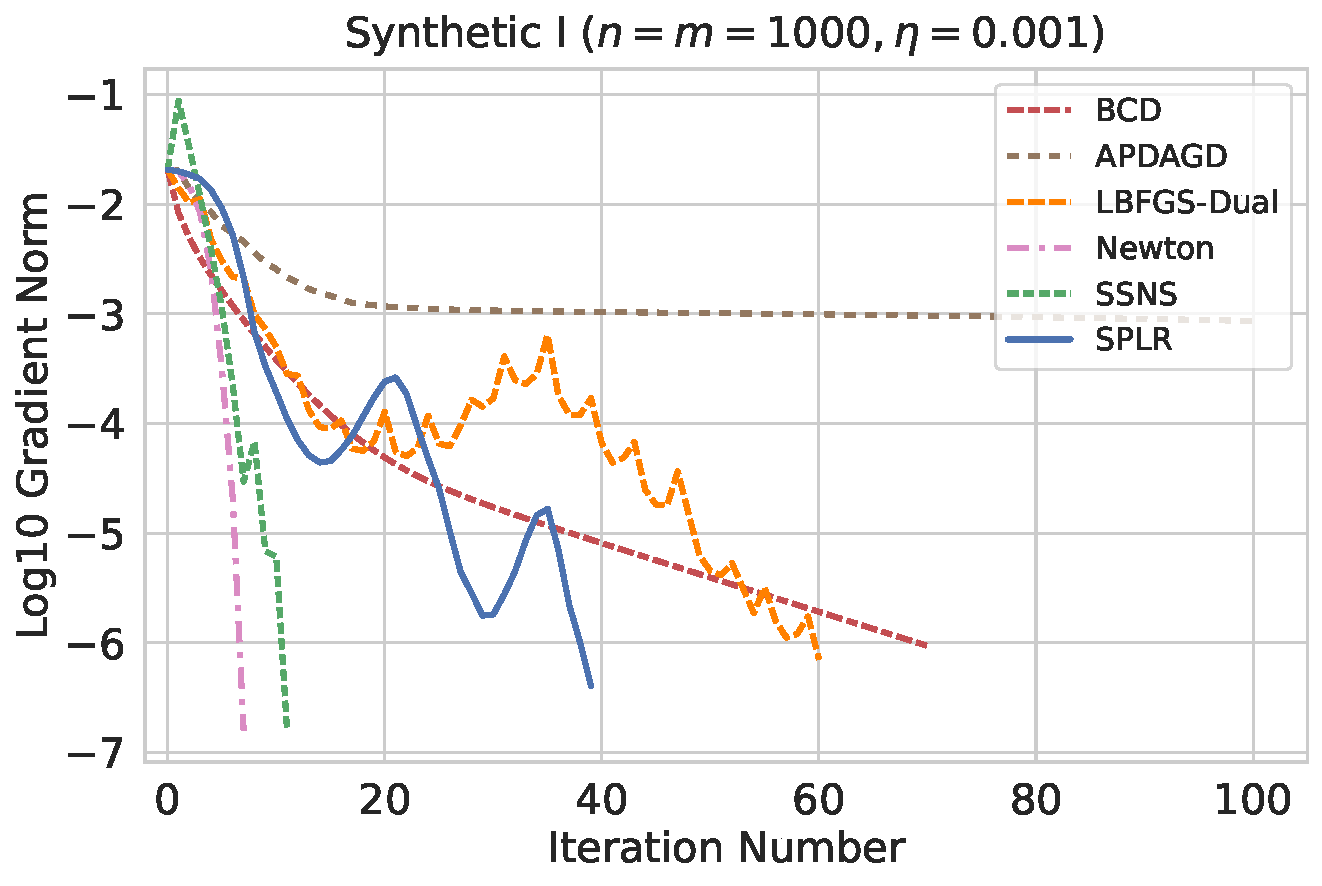
\includegraphics[width=0.3\textwidth]{save/Synthetic I/iterations/n=1000, m=1000, reg=0.001}
        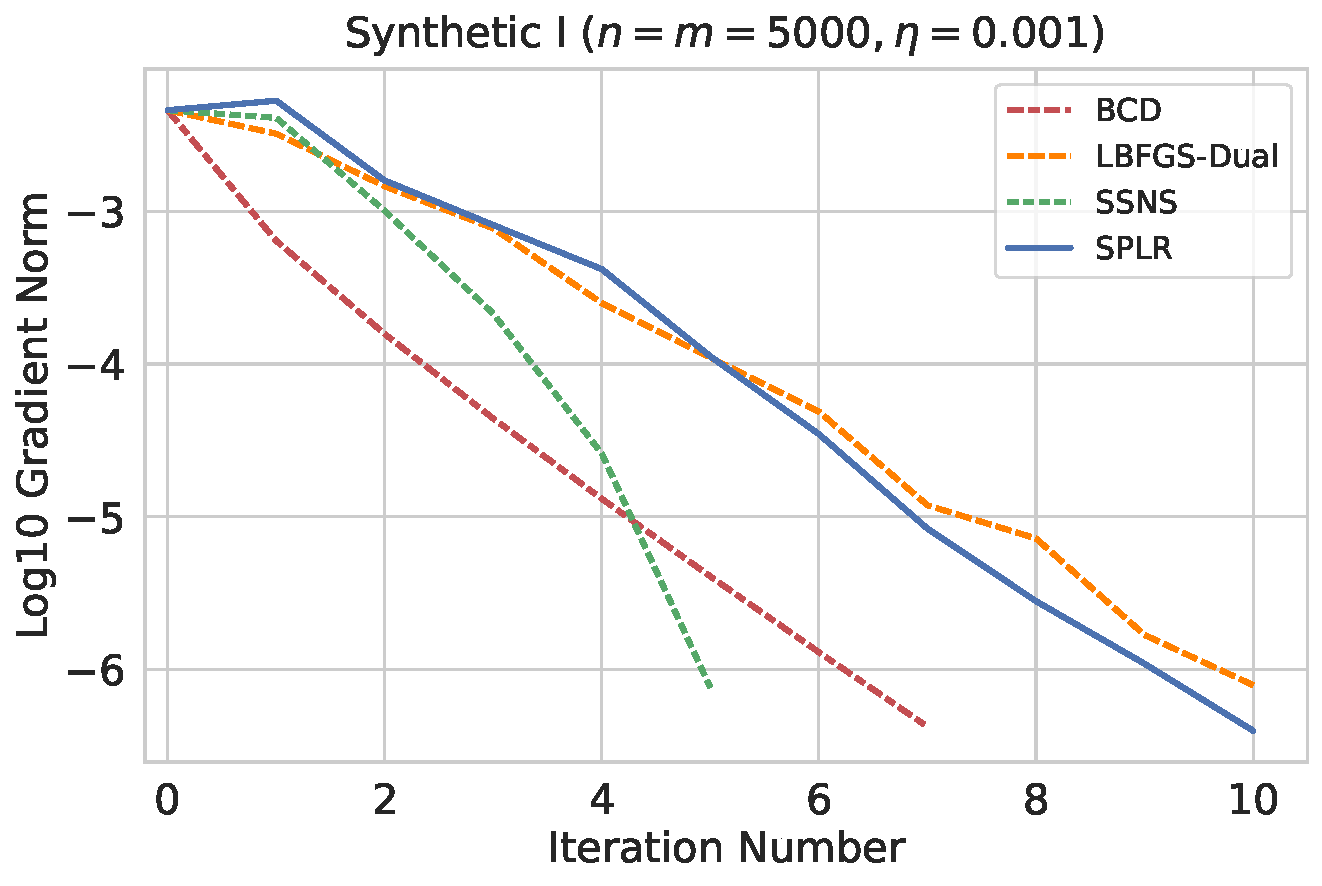
\includegraphics[width=0.3\textwidth]{save/Synthetic I/iterations/n=5000, m=5000, reg=0.001}
        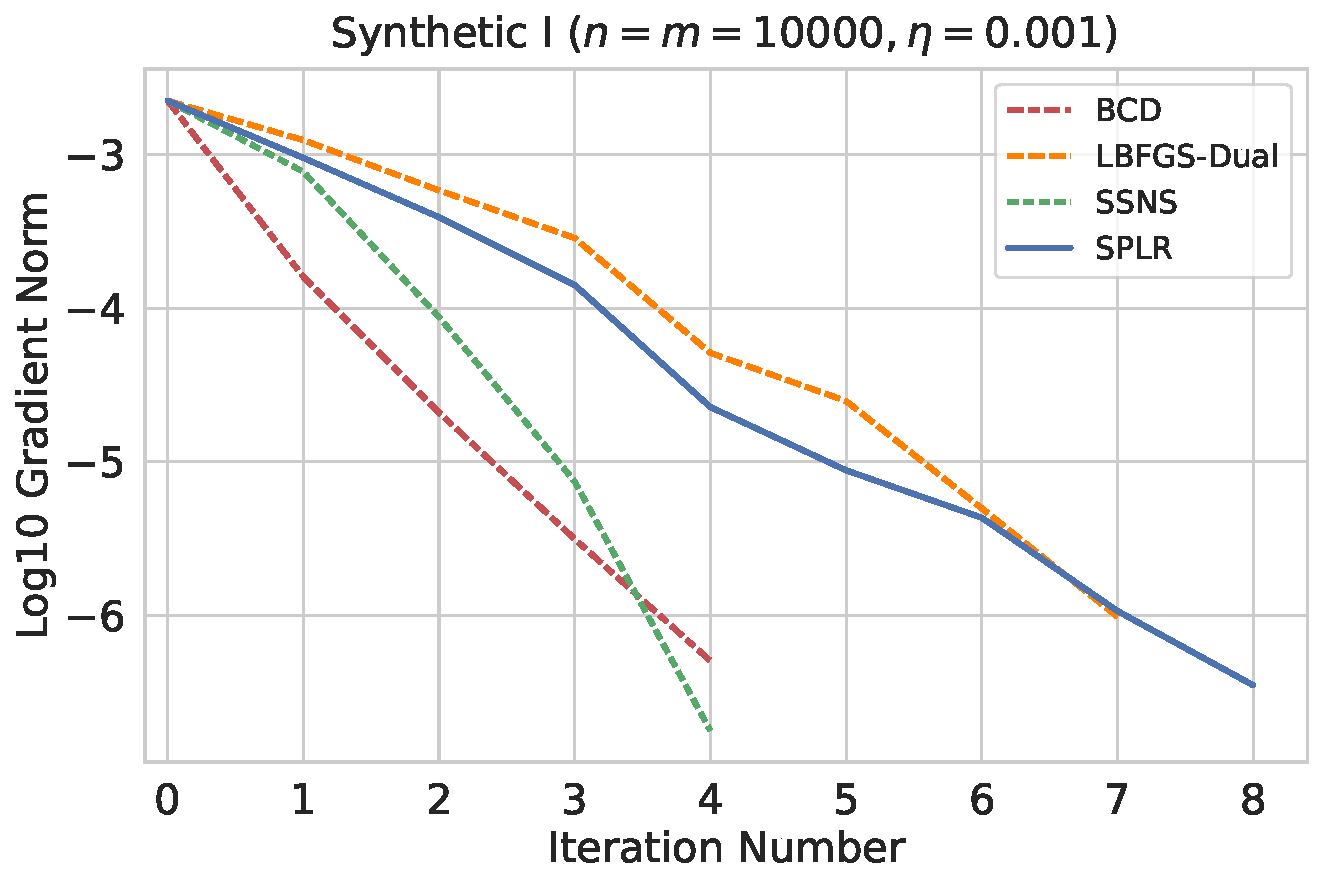
\includegraphics[width=0.3\textwidth]{save/Synthetic I/iterations/n=10000, m=10000, reg=0.001} \\
        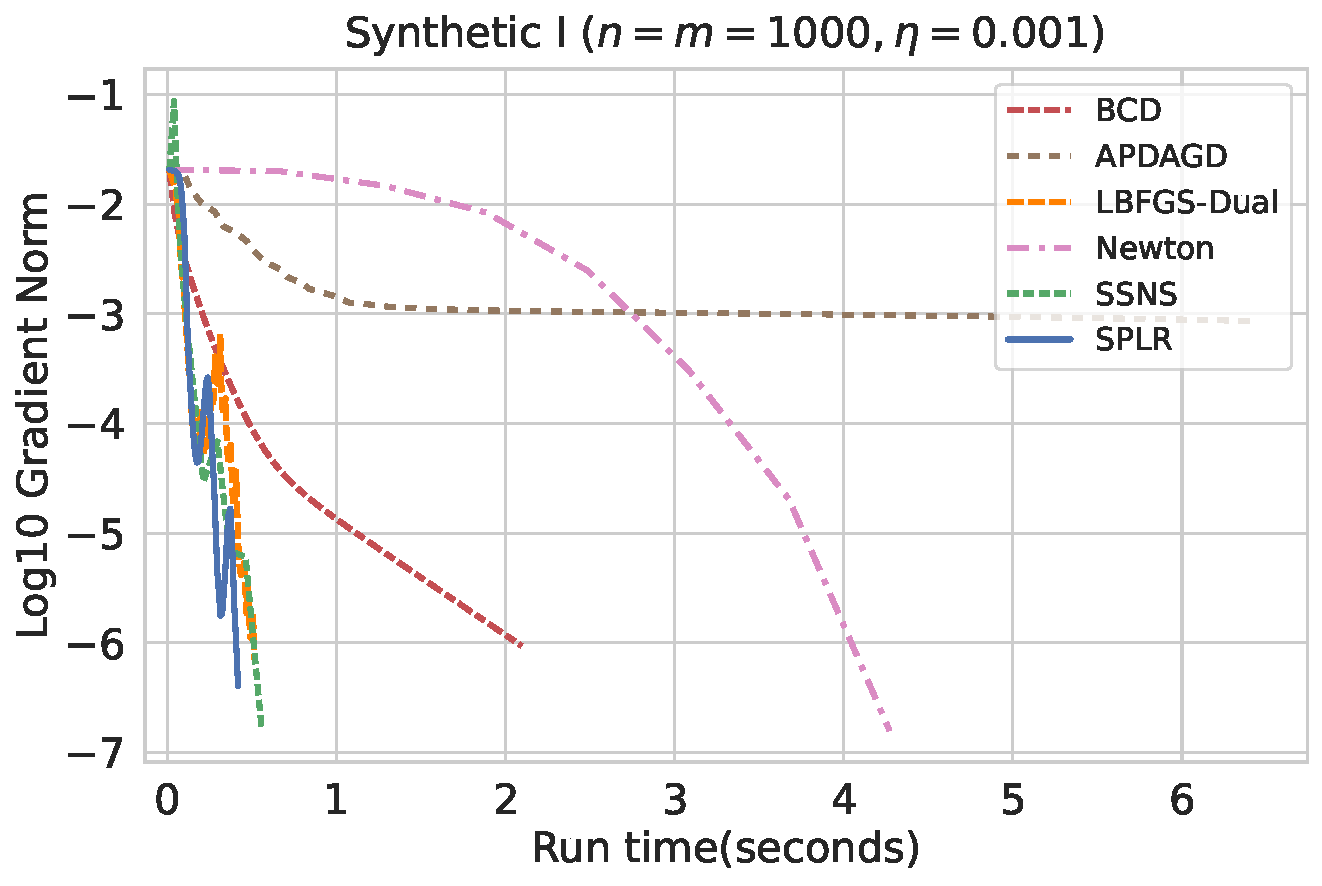
\includegraphics[width=0.3\textwidth]{save/Synthetic I/run_times/n=1000, m=1000, reg=0.001}
        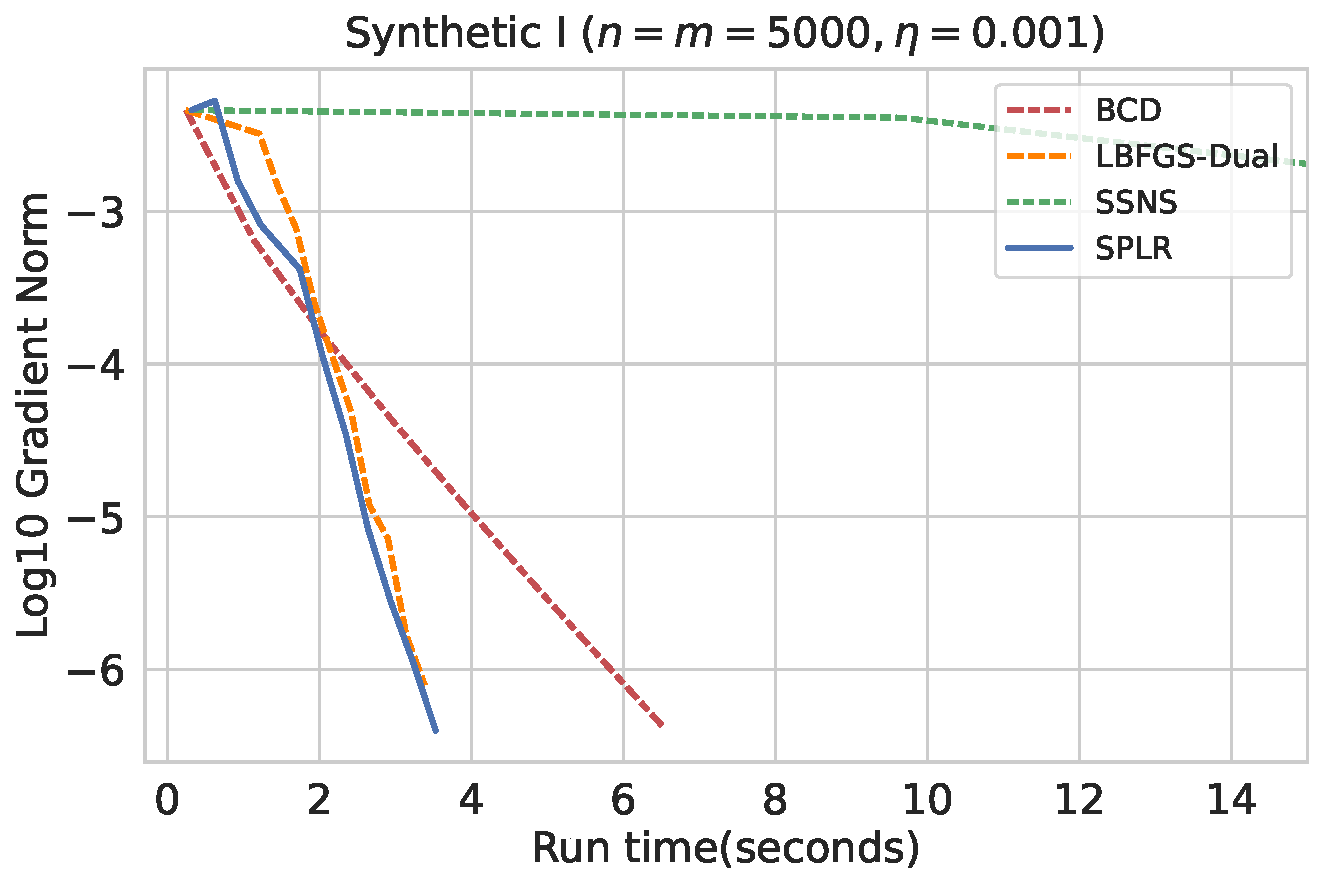
\includegraphics[width=0.3\textwidth]{save/Synthetic I/run_times/n=5000, m=5000, reg=0.001}
        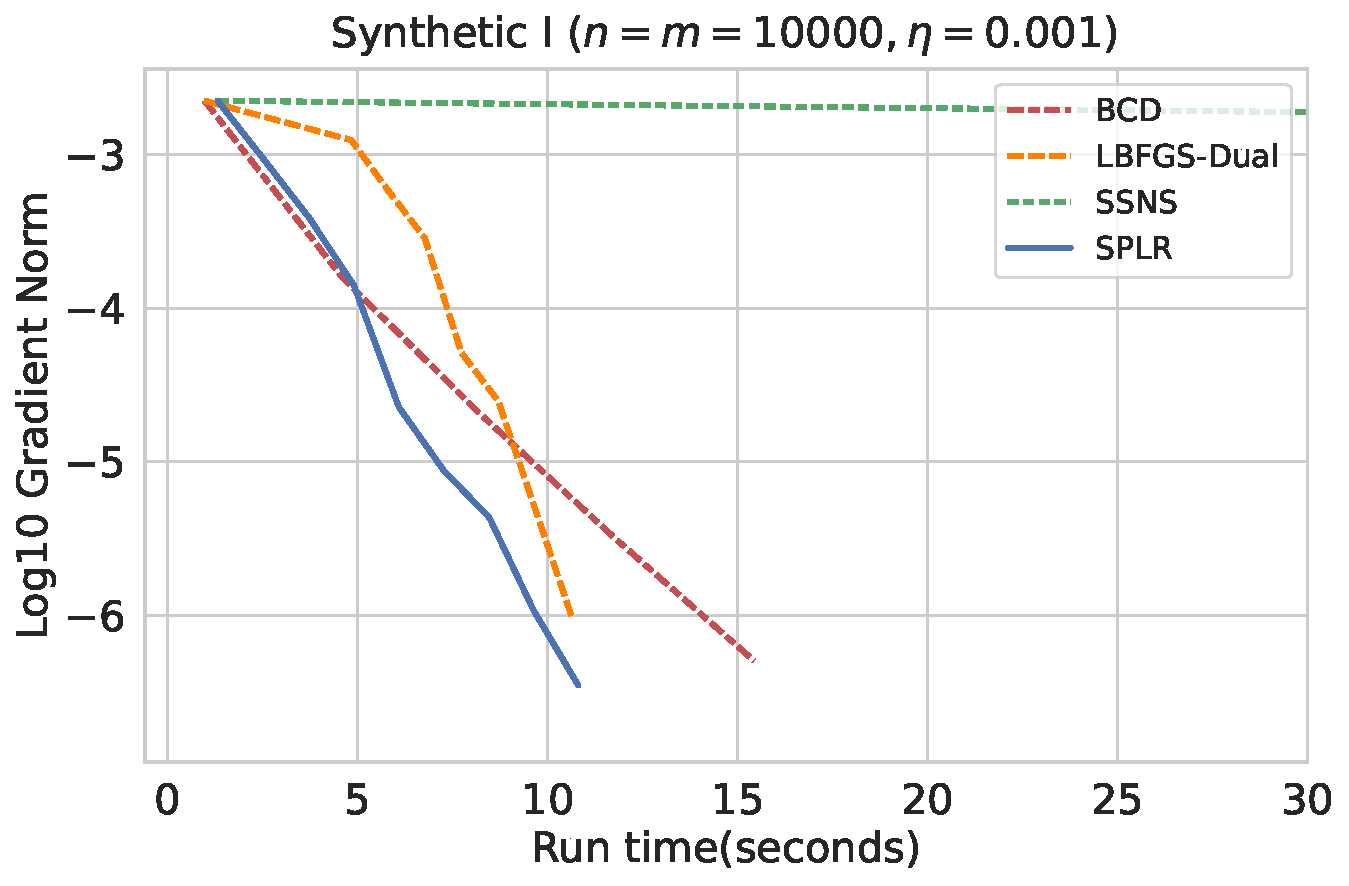
\includegraphics[width=0.3\textwidth]{save/Synthetic I/run_times/n=10000, m=10000, reg=0.001}
        \caption{Top: Gradient norm vs. iteration number. Bottom: Gradient norm vs. run time.}
        \label{fig:synthetic_1}
    \end{figure}
\end{frame}

\begin{frame}{Synthetic II}
    $M_{ij} = (x_i-y_j)^2, a \sim \exp(1), b\sim 0.2\cdot N(1, 0.2) + 0.8 \cdot N(3, 0.5).$

    \begin{figure}
        \centering
        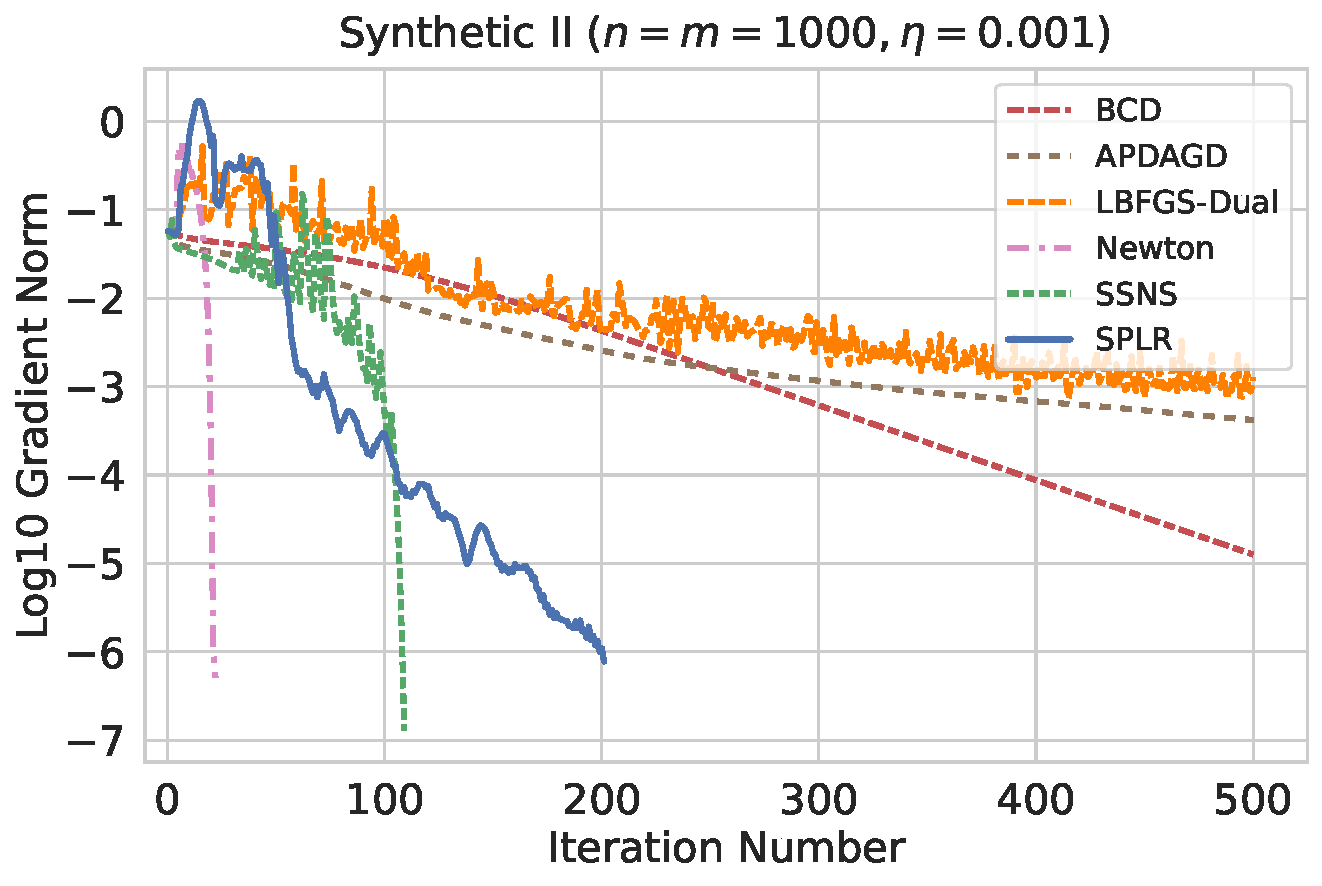
\includegraphics[width=0.3\textwidth]{save/Synthetic II/iterations/n=1000, m=1000, reg=0.001}
        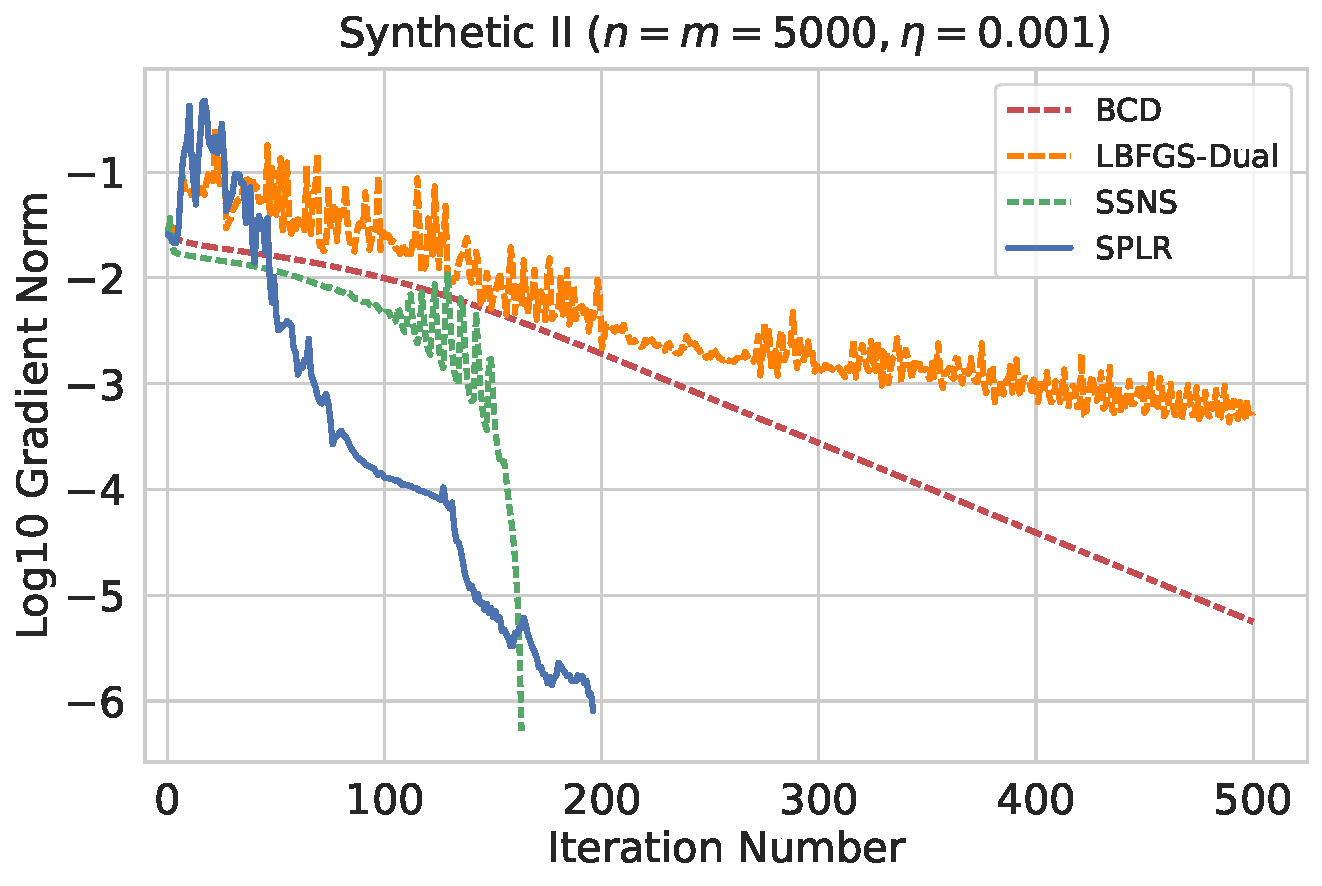
\includegraphics[width=0.3\textwidth]{save/Synthetic II/iterations/n=5000, m=5000, reg=0.001}
        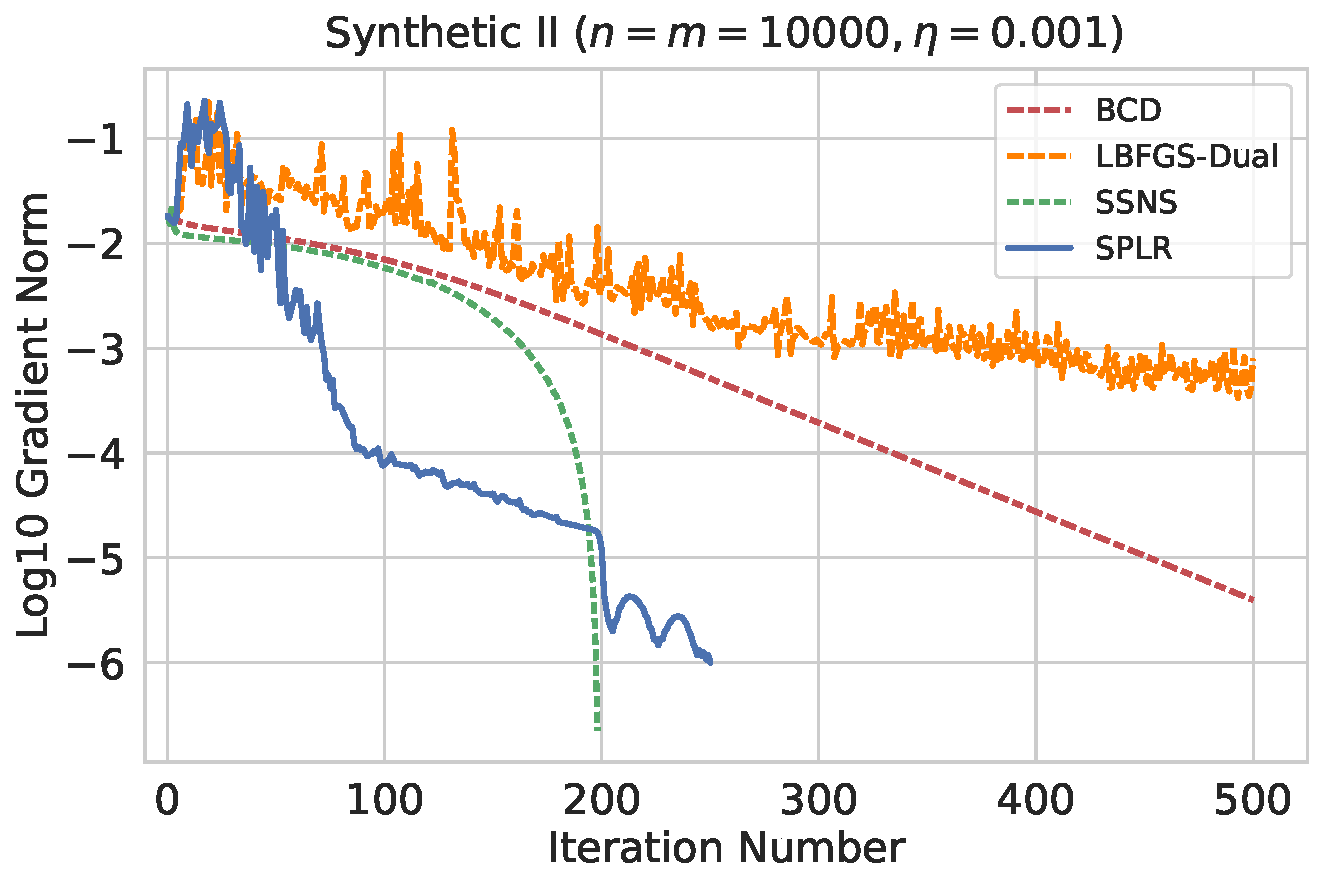
\includegraphics[width=0.3\textwidth]{save/Synthetic II/iterations/n=10000, m=10000, reg=0.001} \\
        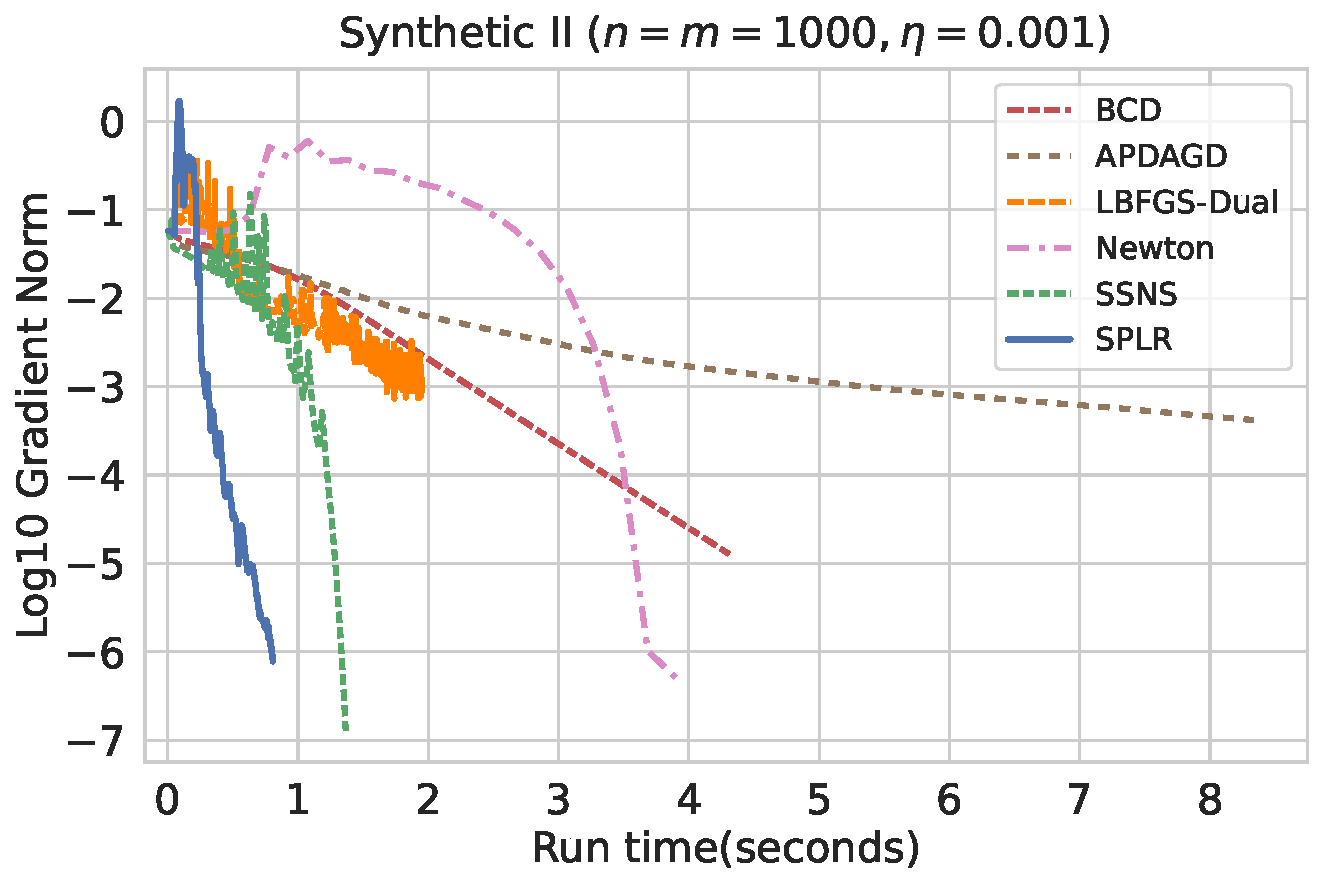
\includegraphics[width=0.3\textwidth]{save/Synthetic II/run_times/n=1000, m=1000, reg=0.001}
        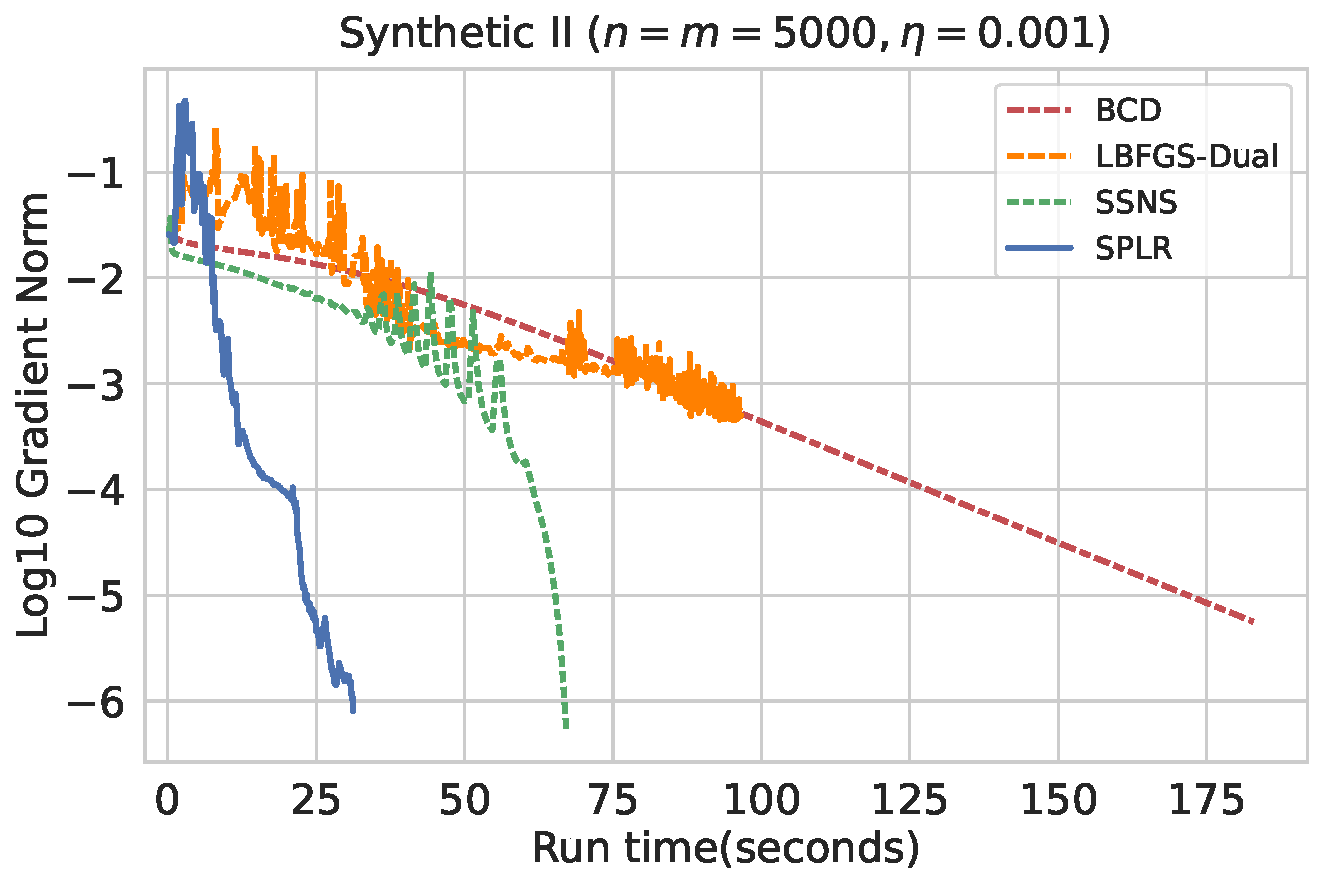
\includegraphics[width=0.3\textwidth]{save/Synthetic II/run_times/n=5000, m=5000, reg=0.001}
        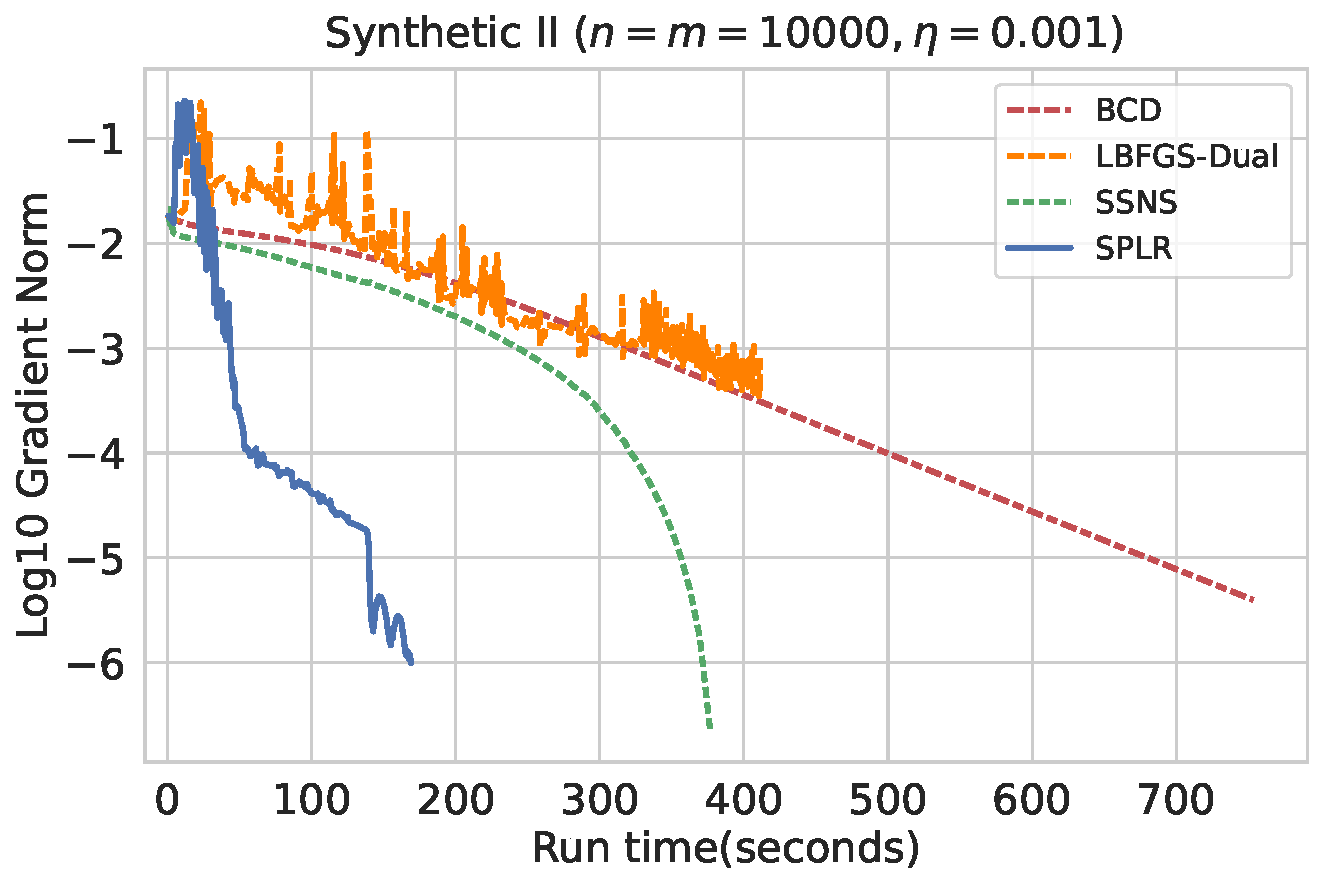
\includegraphics[width=0.3\textwidth]{save/Synthetic II/run_times/n=10000, m=10000, reg=0.001}
        \caption{Top: Gradient norm vs. iteration number. Bottom: Gradient norm vs. run time.}
        \label{fig:synthetic_2}
    \end{figure}
\end{frame}

\begin{frame}{MNIST and Fashion-MNIST}
    \begin{figure}
        \centering
        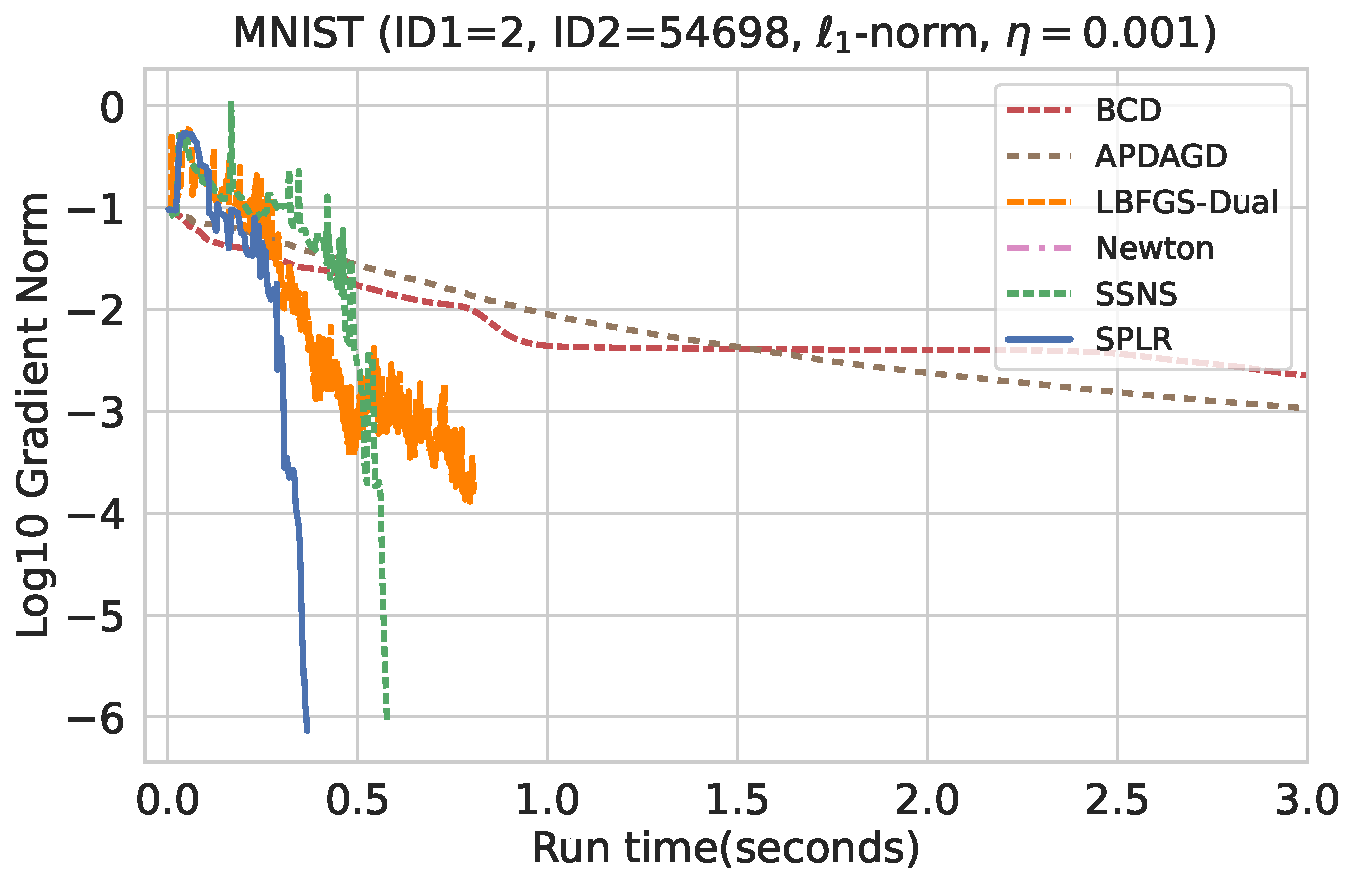
\includegraphics[width=0.3\textwidth]{save/MNIST/run_times/ID1=2, ID2=54698, norm=l1, reg=0.001}
        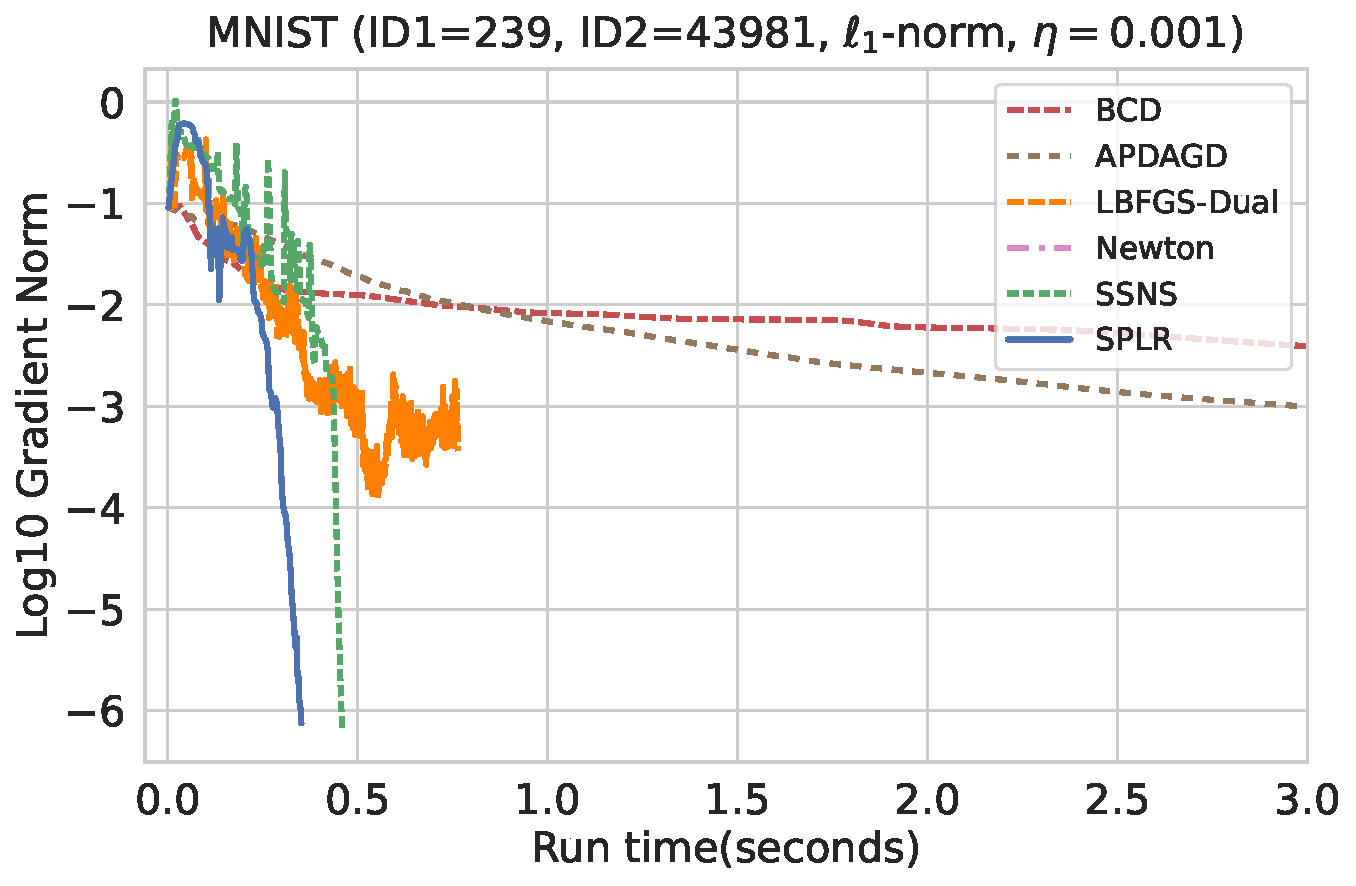
\includegraphics[width=0.3\textwidth]{save/MNIST/run_times/ID1=239, ID2=43981, norm=l1, reg=0.001}
        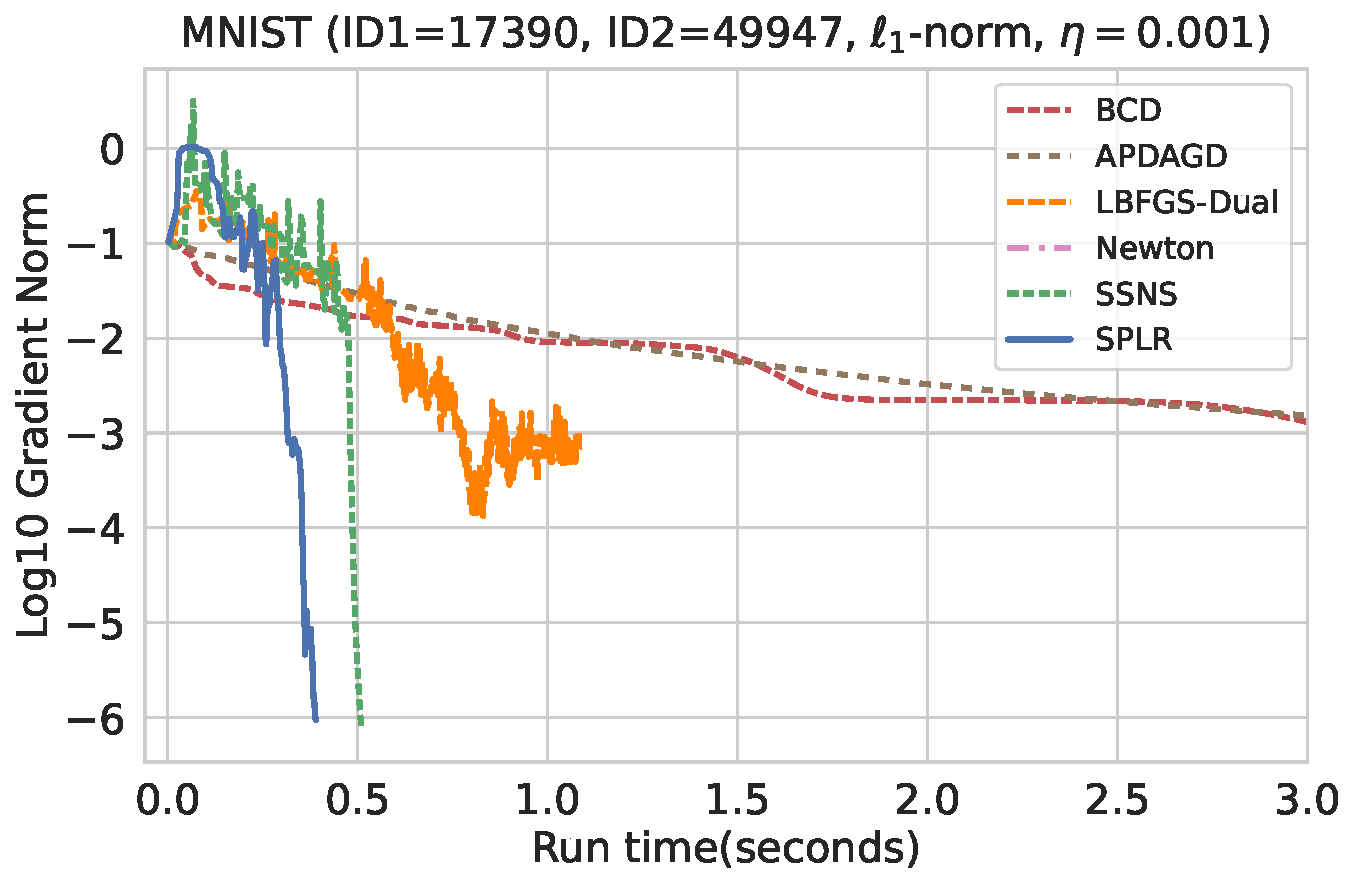
\includegraphics[width=0.3\textwidth]{save/MNIST/run_times/ID1=17390, ID2=49947, norm=l1, reg=0.001}
        \caption{Performance of different algorithms on the MNIST data.}
        \label{fig:mnist}
    \end{figure}
    
    \begin{figure}
        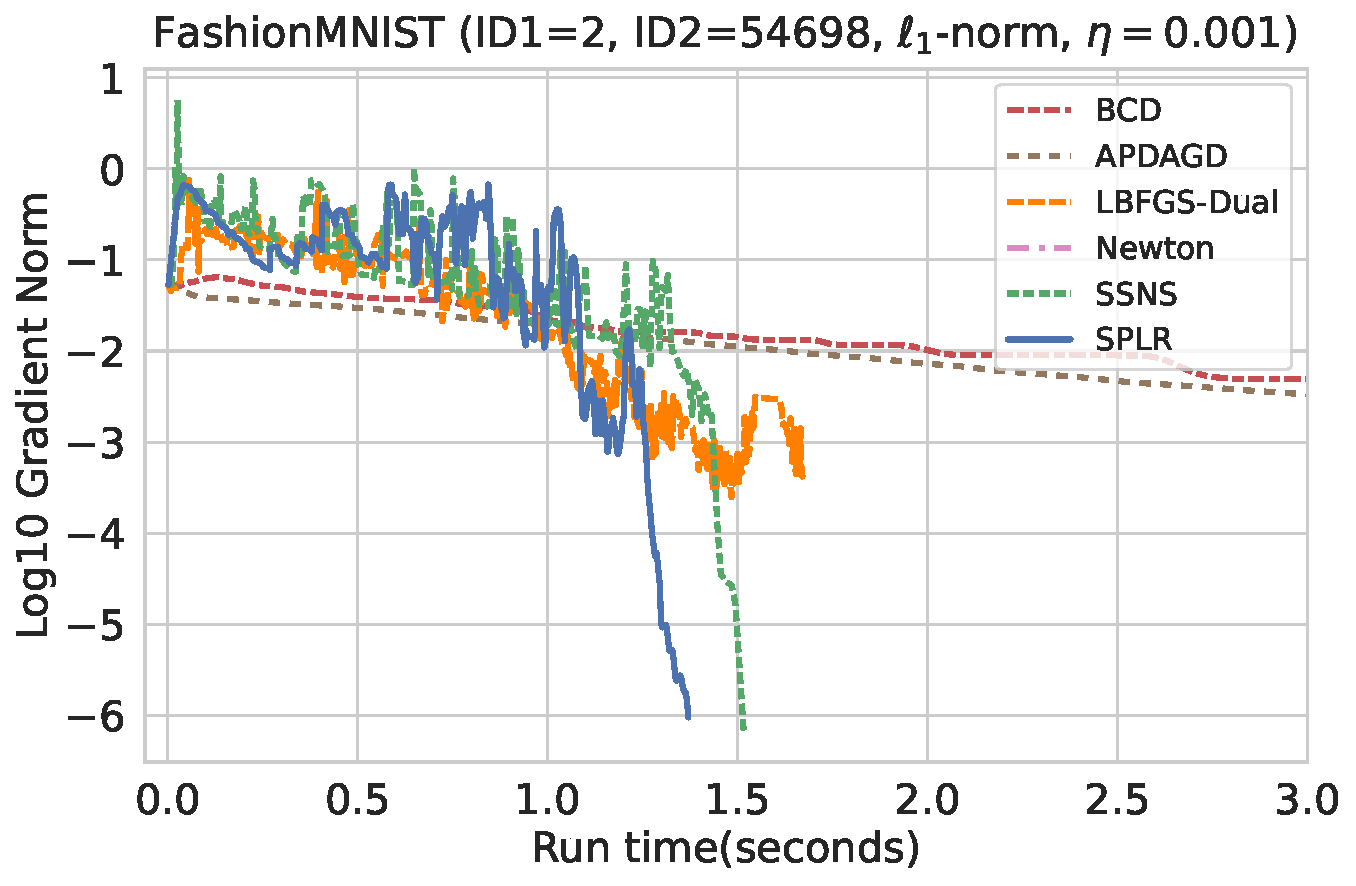
\includegraphics[width=0.3\textwidth]{save/Fashion-MNIST/run_times/ID1=2, ID2=54698, norm=l1, reg=0.001}
        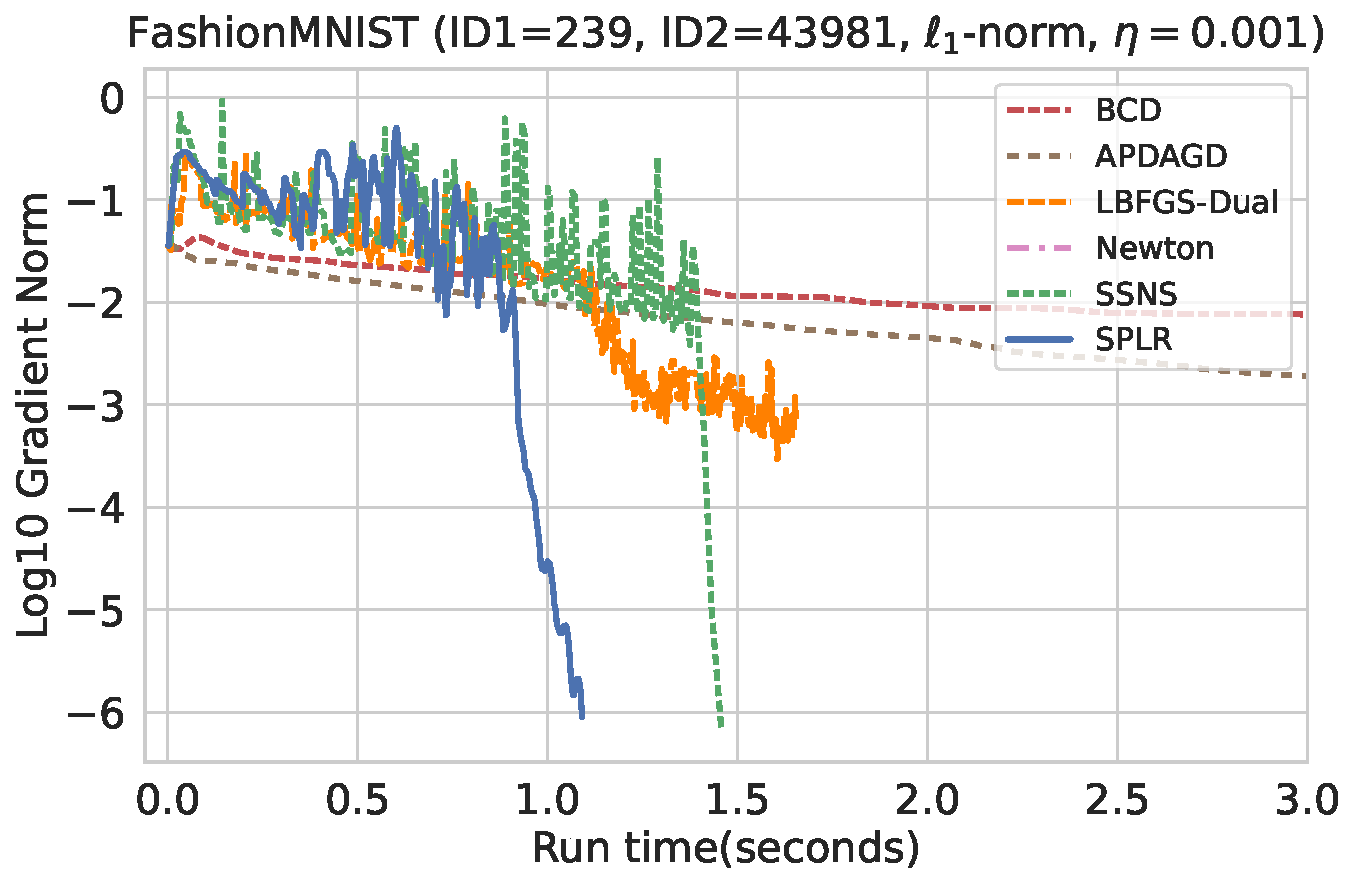
\includegraphics[width=0.3\textwidth]{save/Fashion-MNIST/run_times/ID1=239, ID2=43981, norm=l1, reg=0.001}
        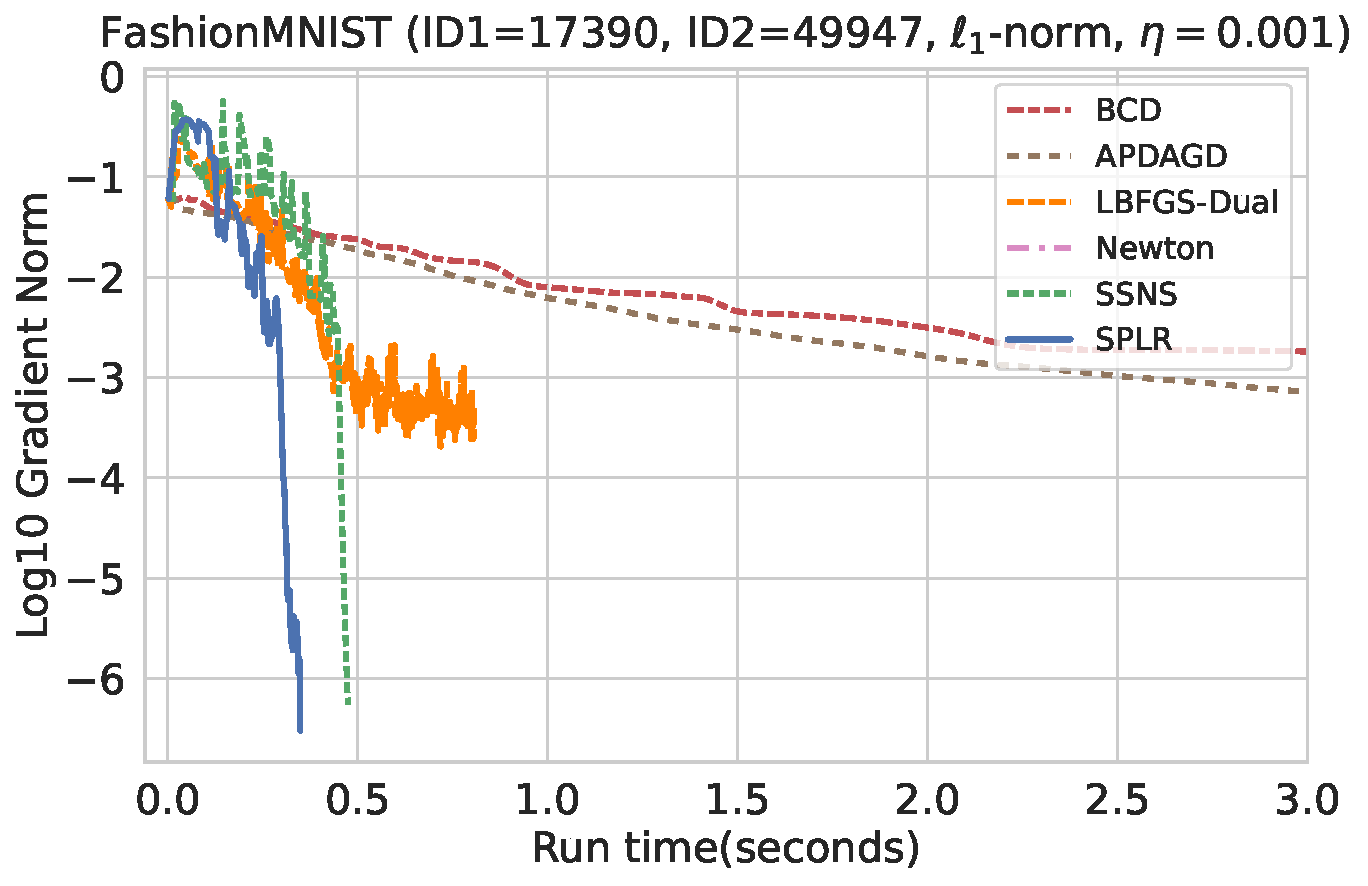
\includegraphics[width=0.3\textwidth]{save/Fashion-MNIST/run_times/ID1=17390, ID2=49947, norm=l1, reg=0.001}
        \caption{Performance of different algorithms on the Fashion-MNIST data.}
        \label{fig:fashion-mnist}
    \end{figure}
\end{frame}

\begin{frame}{ImageNet}
    \begin{figure}[ht]
      \centering
      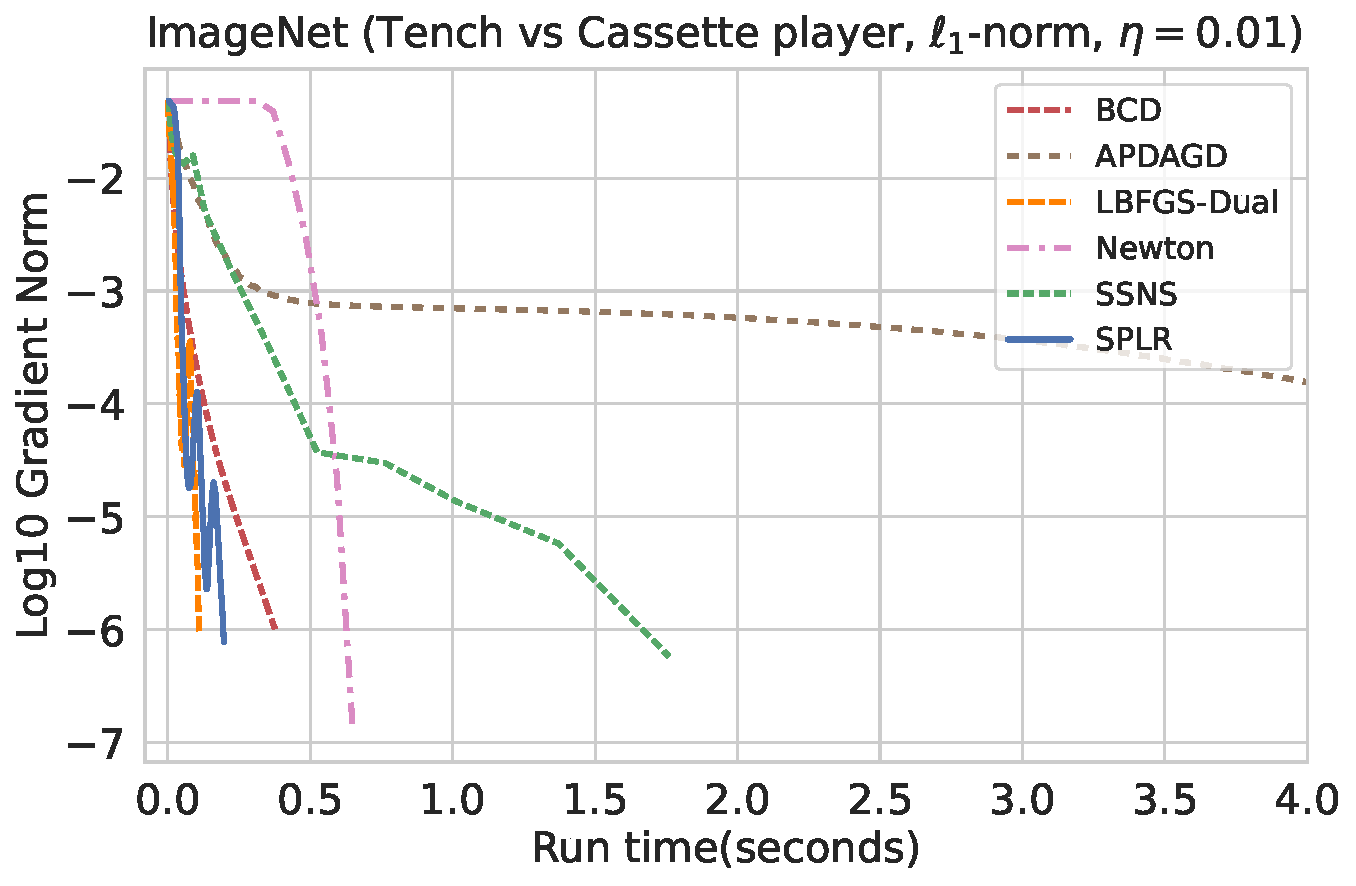
\includegraphics[width=0.4\textwidth]{save/ImageNet/run_times/CLASS1=tench, CLASS2=cassette player, dim=30, norm=l1, reg=0.01}
      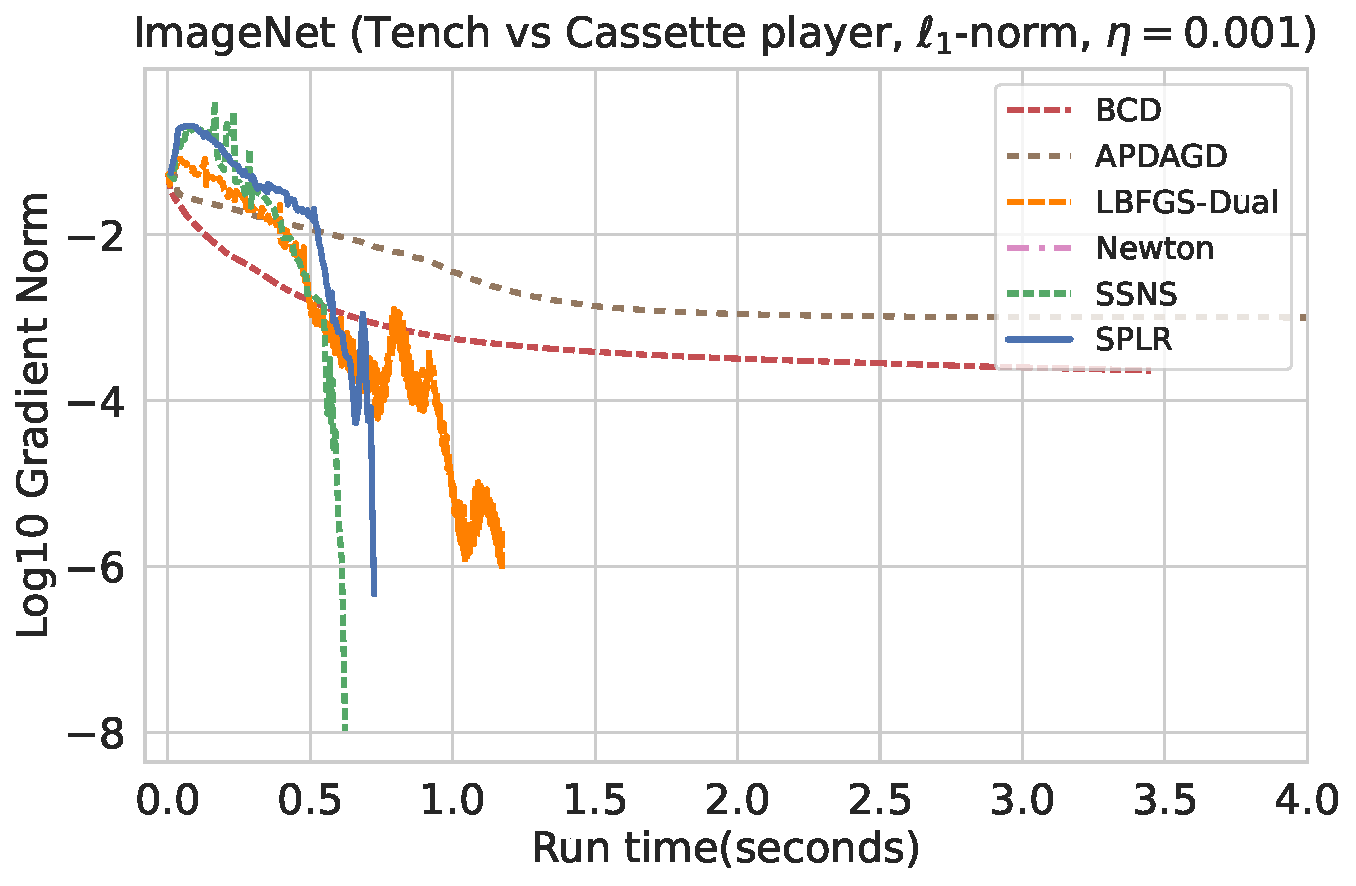
\includegraphics[width=0.4\textwidth]{save/ImageNet/run_times/CLASS1=tench, CLASS2=cassette player, dim=30, norm=l1, reg=0.001}
      \caption{Performance of different algorithms on the ImageNet data. Left: $\eta=0.01$. Right: $\eta=0.001$.}
      \label{fig:imagenet}
    \end{figure}
\end{frame}

\begin{frame}{Ablation Study}
    \begin{figure}[h]
        \centering
        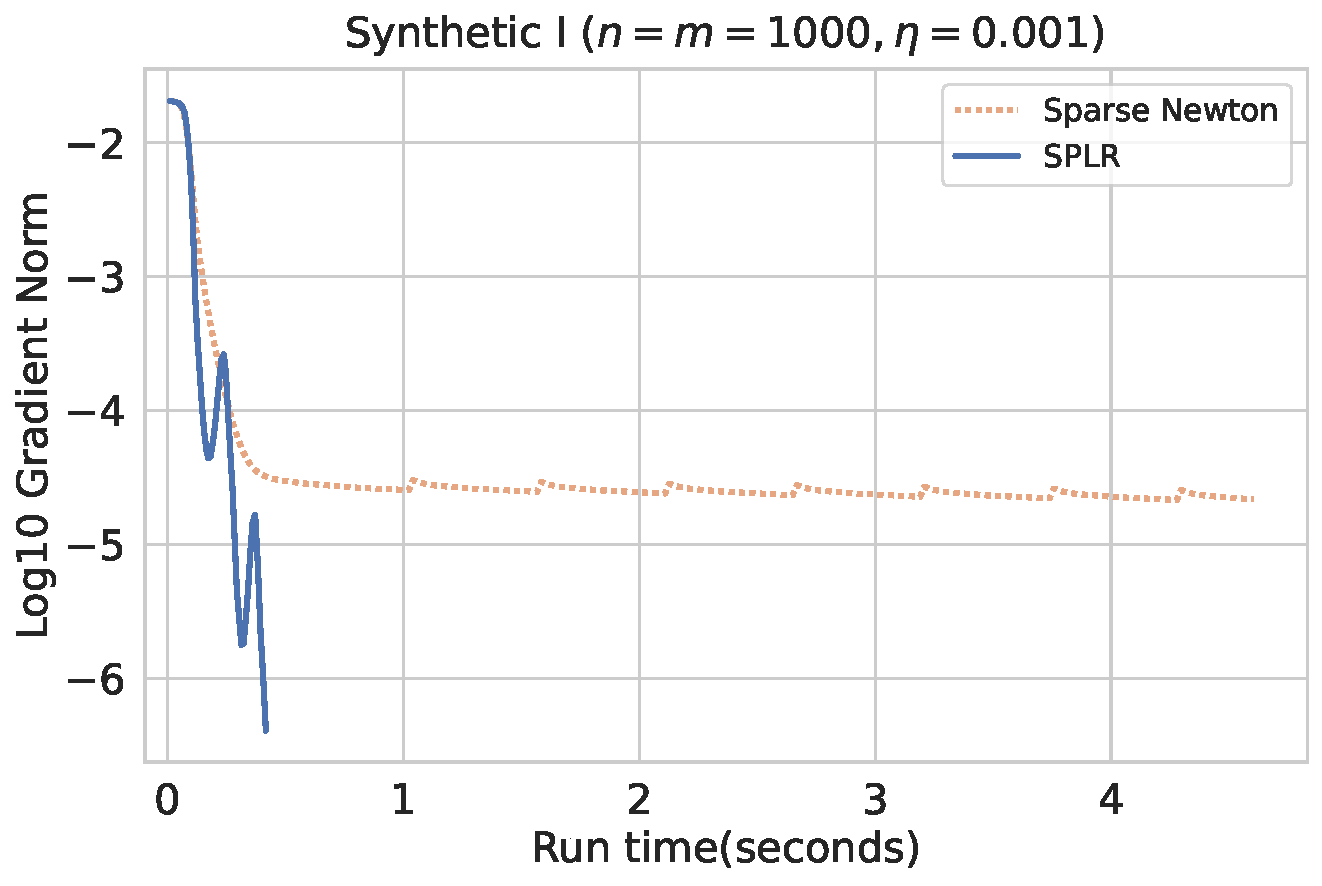
\includegraphics[width=0.3\textwidth]{save/Synthetic I - Ablation/run_times/n=1000, m=1000, reg=0.001}
        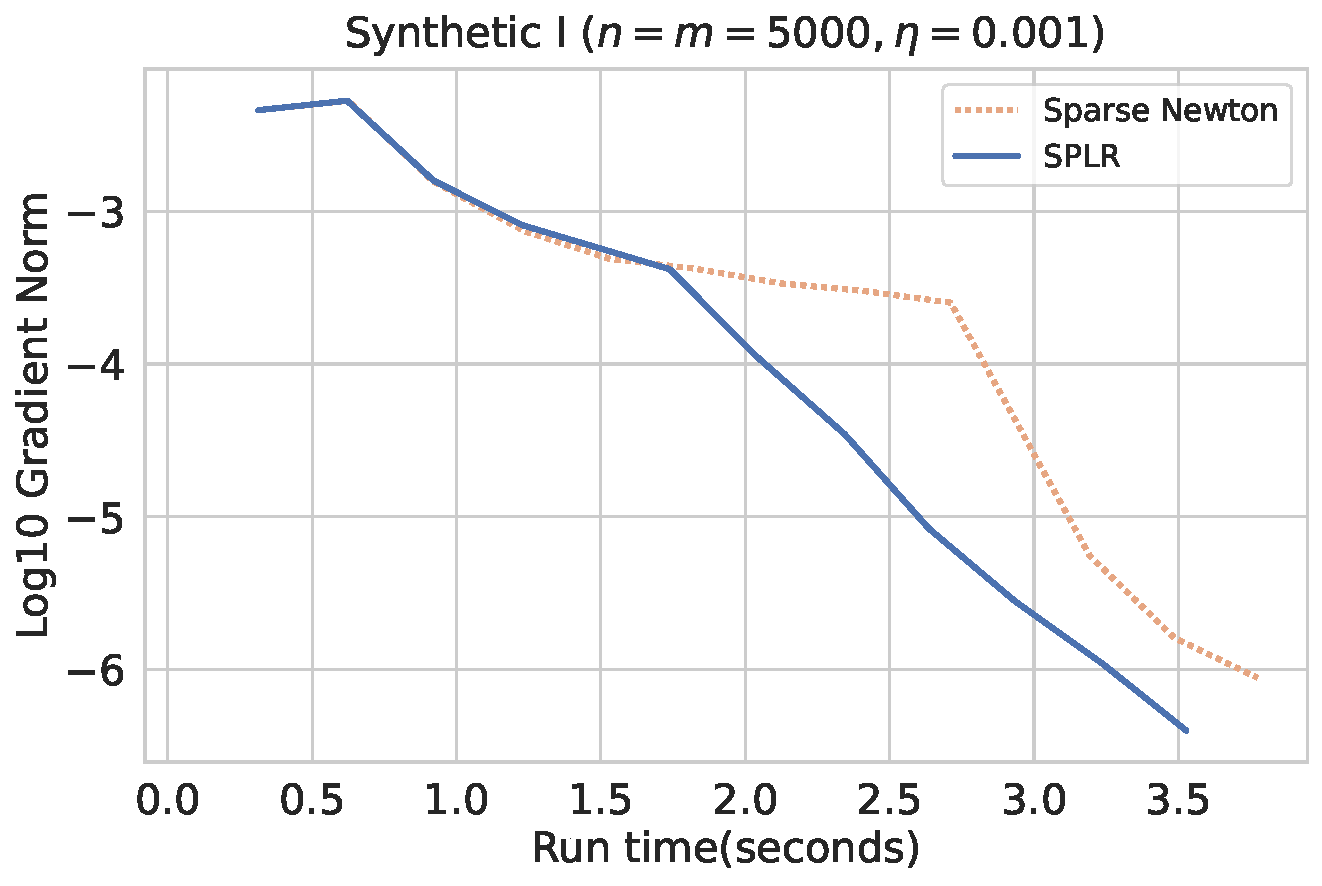
\includegraphics[width=0.3\textwidth]{save/Synthetic I - Ablation/run_times/n=5000, m=5000, reg=0.001}
        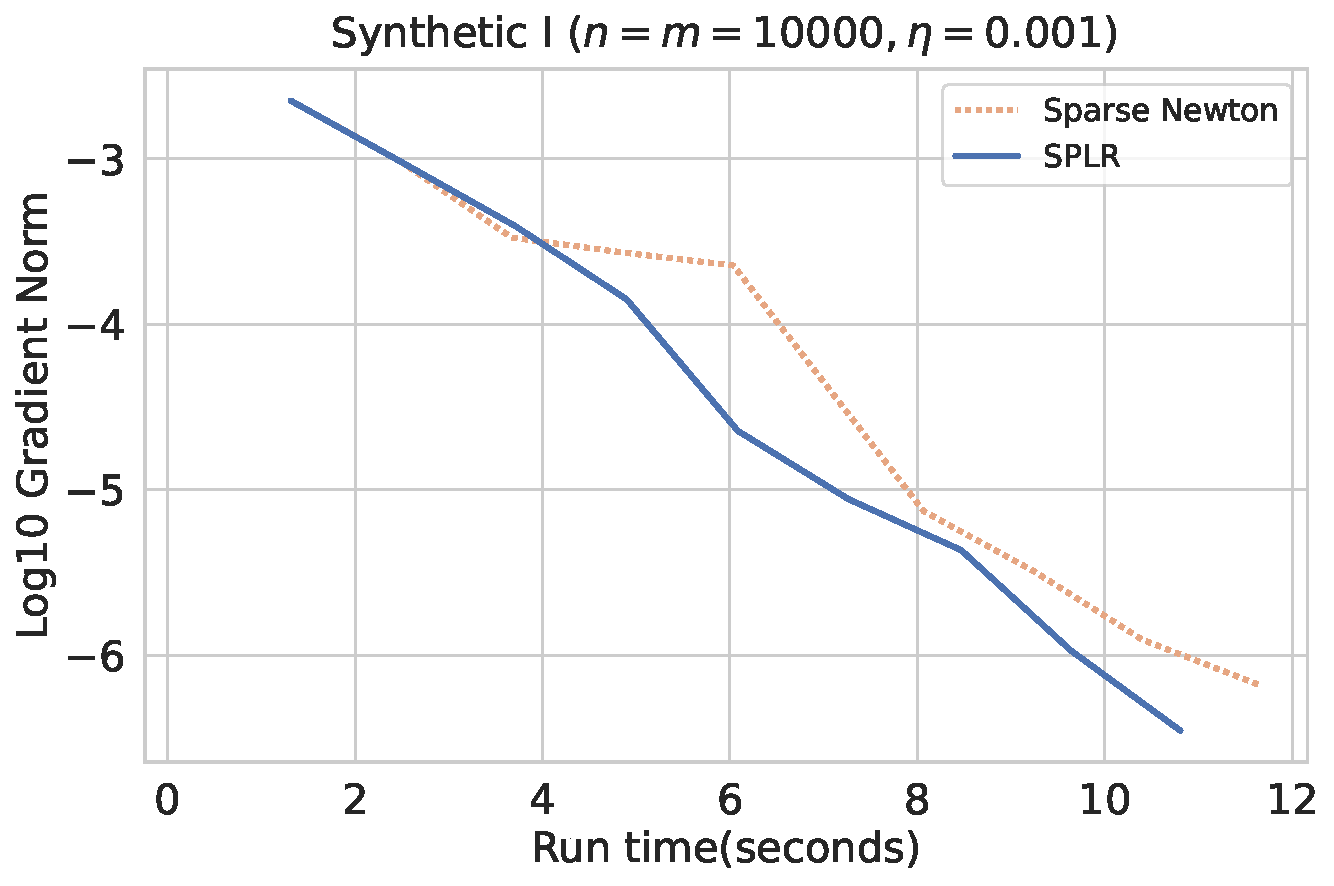
\includegraphics[width=0.3\textwidth]{save/Synthetic I - Ablation/run_times/n=10000, m=10000, reg=0.001} \\
        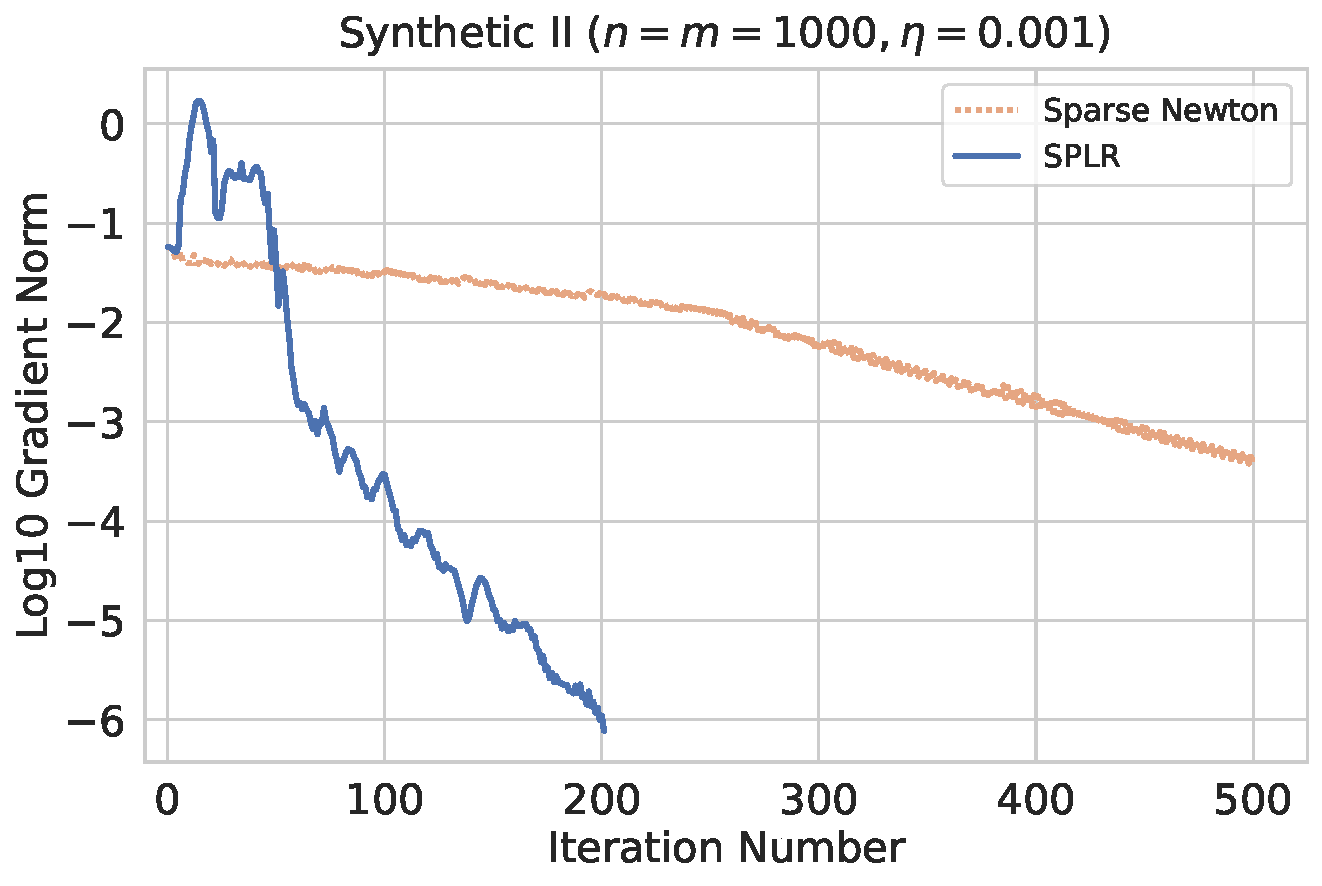
\includegraphics[width=0.3\textwidth]{save/Synthetic II - Ablation/iterations/n=1000, m=1000, reg=0.001.pdf}
        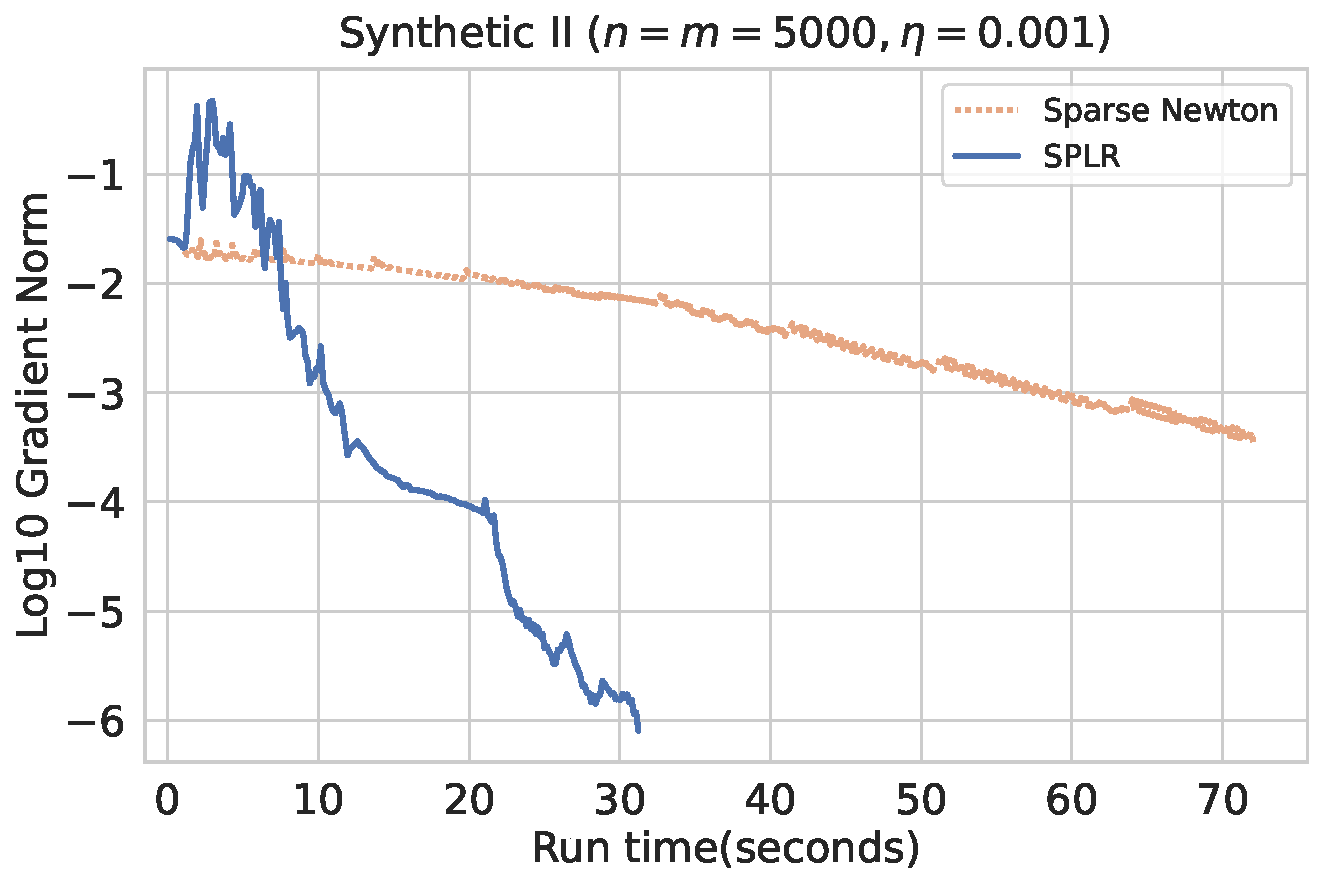
\includegraphics[width=0.3\textwidth]{save/Synthetic II - Ablation/run_times/n=5000, m=5000, reg=0.001.pdf}
        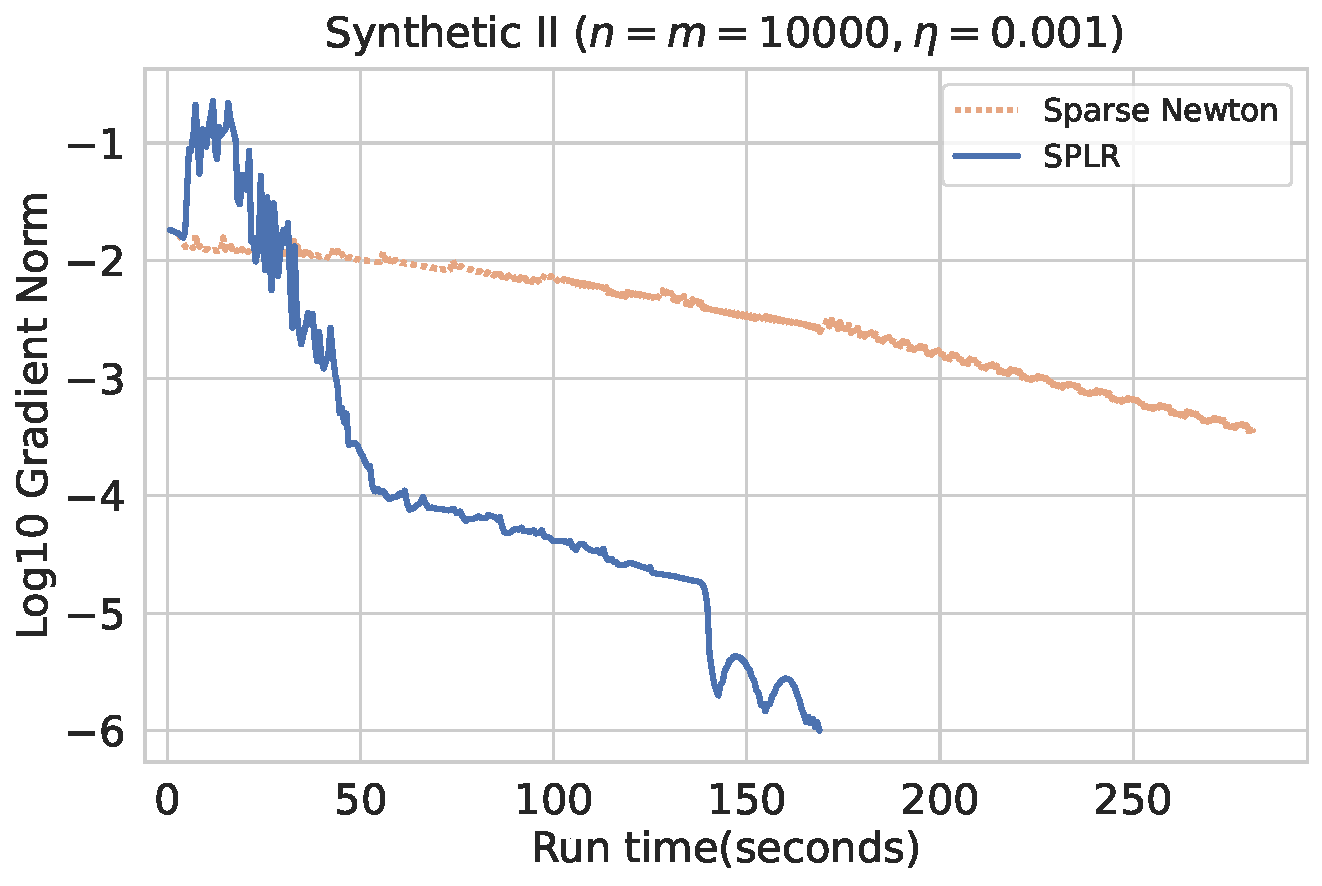
\includegraphics[width=0.3\textwidth]{save/Synthetic II - Ablation/run_times/n=10000, m=10000, reg=0.001.pdf}
        \caption{Top: Synthetic I. Bottom: Synthetic II.}
        \label{fig:effect_low_rank_i}
    \end{figure}
\end{frame}